%%%%%%%%%%%%%%%%%%%%%%%%%%%%%%%%%%%%%%%%%%%%%%%%%%%%%%%%%% 
\chapter{グラフ彩色問題とその関連問題}\label{chap:background}
%%%%%%%%%%%%%%%%%%%%%%%%%%%%%%%%%%%%%%%%%%%%%%%%%%%%%%%%%%

%%%%%%%%%%%%%%%%%%%%%%%%%%%%%%%%%
\begin{figure}[t]
  \begin{tabular}{cc}
    \begin{minipage}[t]{0.5\linewidth}
      \centering
      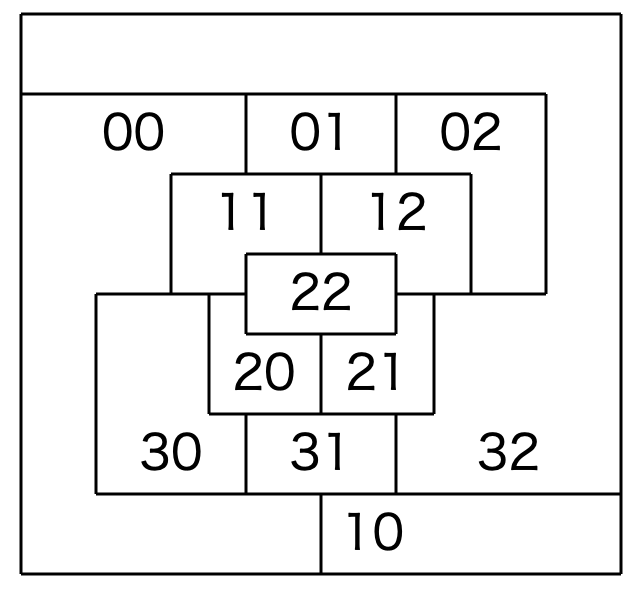
\includegraphics[keepaspectratio,clip,scale=0.23]{fig/order3.png}
      \caption{3次の\code{McGregor}グラフ}
      \label{fig:order3}
    \end{minipage}
    \begin{minipage}[t]{0.5\linewidth}
      \centering
      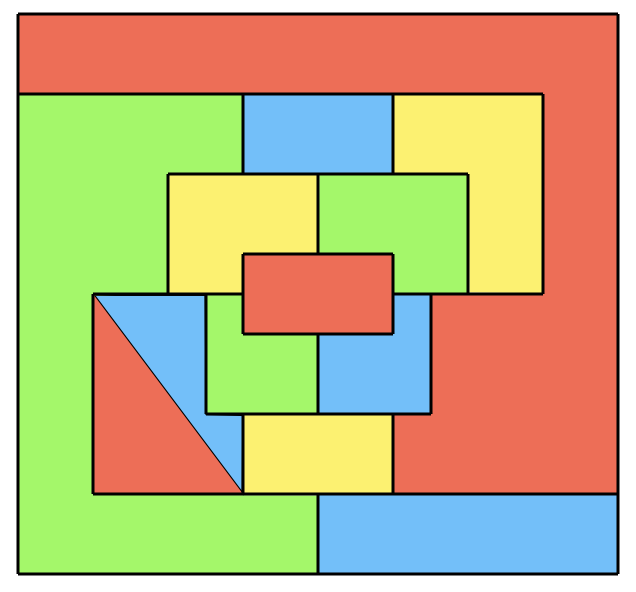
\includegraphics[keepaspectratio,clip,scale=0.23]{fig/order3_mult.png}
      \caption{3次の\code{McGregor}グラフに対する多色頂点数最大化問題の最適解}
      \label{fig:order3mult}
    \end{minipage}
  \end{tabular}
\end{figure}
%%%%%%%%%%%%%%%%%%%%%%%%%%%%%%%%%
%%%%%%%%%%%%%%%%%%%%%%%%%%%%%%%%% 
\begin{figure}[t]
  \centering
  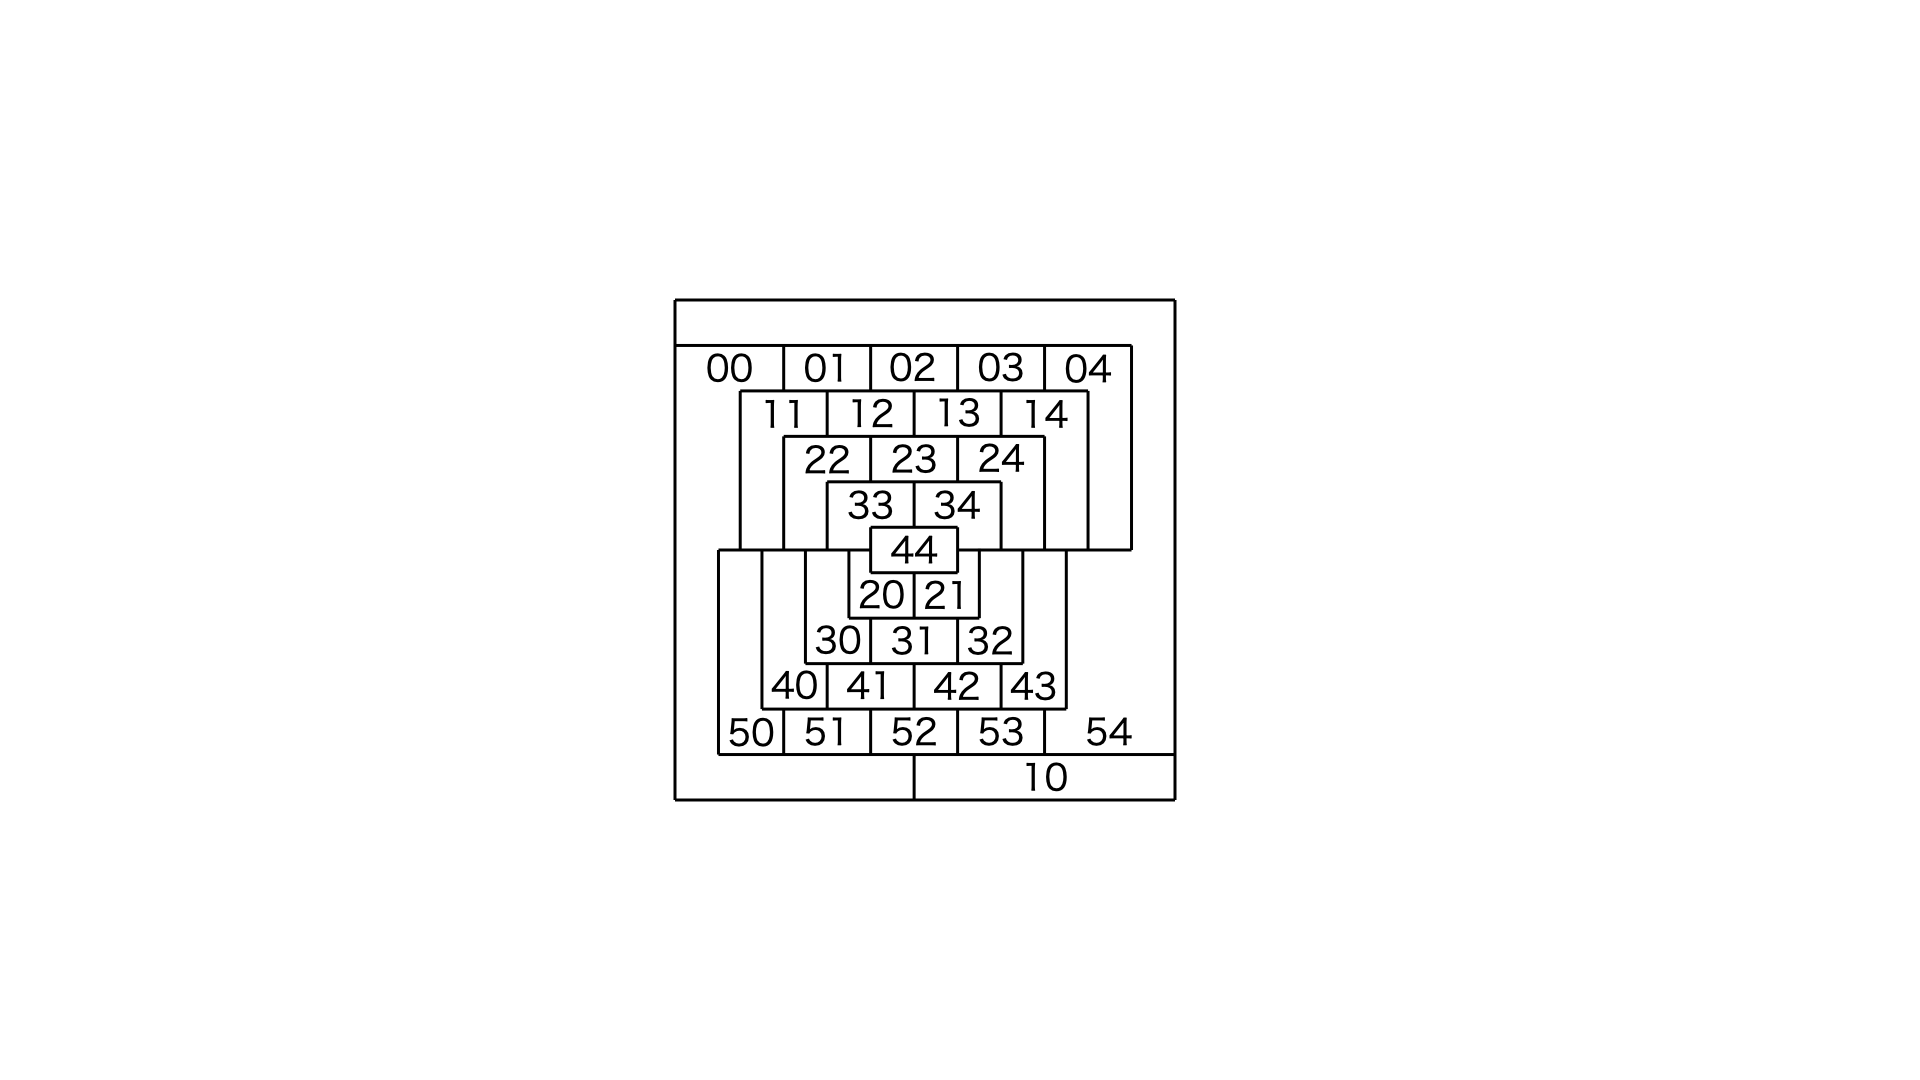
\includegraphics[keepaspectratio,clip,scale=0.4]{fig/order5.png}
  \caption{5次の\code{McGregor}グラフ}
  \label{fig:order5}
\end{figure}
%
\begin{figure}[t]
  \centering
  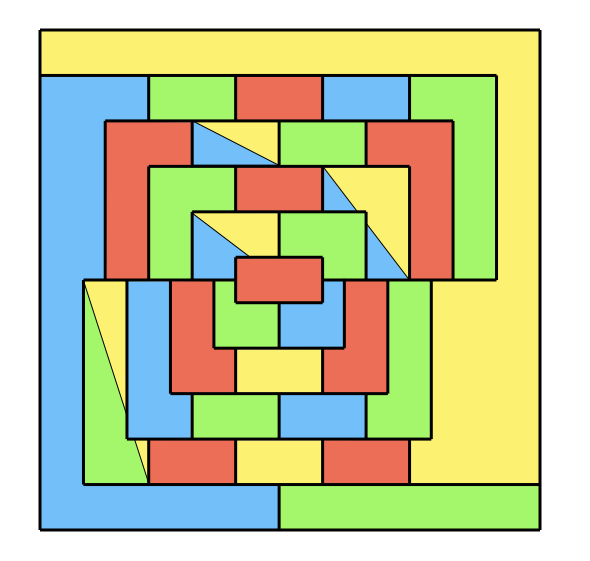
\includegraphics[keepaspectratio,clip,scale=0.4]{fig/order5_mult.png}
  \caption{5次の\code{McGregor}グラフに対する多色頂点数最大化問題の最適解}
  \label{fig:order5mult}
\end{figure}
%%%%%%%%%%%%%%%%%%%%%%%%%%%%%%%%%

\textbf{グラフ彩色問題} (Graph Coloring Problem; GCP)は,
与えられた有限無向グラフ$G$について,隣接する頂点が同色にならない
ように各頂点を塗りわけるとき,必要となる最小の色数
(\textbf{彩色数}と呼ばれる)を求める問題である.
グラフ彩色問題はNP困難な問題であり,最適化コンパイラのレジスタ割
り付けや無線の周波数割り当て等の応用がある.
自然数$k\geq 3$について,グラフ$G$が$k$色以下で彩色可能かどう
かを決定する\textbf{グラフ彩色判定問題}はNP完全である.
$G$が$k$色以下で彩色可能で,$k-1$色以下で彩色可能でないとき,
$G$の彩色数は$k$となる.

本論文では,以下に挙げるグラフ彩色に関する最適化問題を対象とする.
これらの問題は,Knuth の教科書 The Art of Computer Programming (TAOCP)
でも取り上げられている~\cite{Knuth:TAOCP:SAT}.

\begin{itemize}
\item \textbf{同色頂点数最小化問題: }\\
  グラフ彩色判定問題の実行可能解のうち,同色(例えば,赤色)で塗られる
  頂点数の最小値を求める問題である.
\item \textbf{同色頂点数最大化問題: }\\
  グラフ彩色判定問題の実行可能解のうち,同色(例えば,赤色)で塗られる
  頂点数の最大値を求める問題である.
\item \textbf{多色頂点数最大化問題: }\\
  グラフ彩色判定問題の制約を満たしつつ,
  多色(2色以上)で塗られる頂点数の最大値を求める問題である.
  この問題の最適解は,基のグラフ彩色判定問題の複数の実行可能解に対応す
  るため,基の問題の圧縮解とみなすことができる.
\end{itemize}

多色頂点数最大化問題の例として,
3次の\code{McGregor}グラフ(図~\ref{fig:order3})と
その最適解の一例(図~\ref{fig:order3mult})を示す.
\code{McGregor}グラフは,各区画が頂点に,
区画の隣接関係が辺に対応する.
3次の\code{McGregor}グラフは12個の頂点と30個の辺
から構成される.
図~\ref{fig:order3mult}は,$k=4$の多色頂点数最大化問題の最適解であり,
その最適値は1である.図から頂点番号\code{30}が
多色(赤あるいは青)で彩色できることがわかる.
これは,赤と青のどちらかがグラフ彩色の制約を満たすのではなく,
赤と青のどちらでも制約を満たすことを意味する.
よって,この最適解は,基の$k=4$のグラフ彩色判定問題の
2つの実行可能解に対応するため,基の問題の圧縮解とみなすことができる.
%
同様に,5次の\code{McGregor}グラフ(図~\ref{fig:order5})と
その最適解の一例(図~\ref{fig:order5mult})を示す.
最適値は4で,
頂点番号\code{12}, \code{24}, \code{33}, \code{50}
の4箇所が2色で彩色できることがわかる.
したがって,図~\ref{fig:order5mult}の最適解は,
$k=4$のグラフ彩色判定問題における
16個の実行可能解の圧縮解とみなすことができる.

\code{McGregor}グラフは,Knuth の TAOCP でもグラフ彩色に関する練習問題
として使われている~\cite{Knuth:TAOCP:SAT}.
また,10次の\code{McGregor}グラフは,
Scientific American の1975年4月号で,
Martin Gardner が塗り分けには5色が必要と紹介し世間を驚かせた
\footnote{エイプリルフールのジョーク}.

%%% Local Variables:
%%% mode: latex
%%% TeX-master: "paper"
%%% End:
